%
%===============>>  ПРОБНИК 3 <<=============
%

%BEGIN_FOLD % ====>>_____ Вариант 1 _____<<====
\begin{training}
	\title{Часть 1}
	\egepreambone
	\begin{listofex}
		%1
		\item
		\begin{minipage}[t]{\bodywidth}
			Радиус окружности, описанной около правильного треугольника, равен \( 3 \). Найдите высоту этого треугольника.
			\foranswer
		\end{minipage}
		\gapwidth
		\begin{minipage}[t]{\picwidth}
			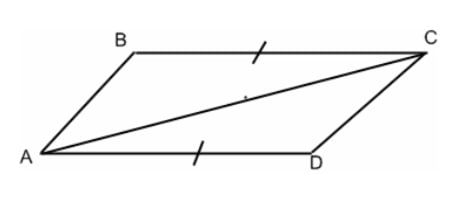
\includegraphics[align=t, width=\linewidth]{\picpath/../../bank/graphs/graph_gleb/probniki_21.04/n1v1}
		\end{minipage}
		%2
		\item
		\begin{minipage}[t]{\bodywidth}
			Объем параллелепипеда \( ABCDA_1B_1C_1D_1 \) равен \( 9 \). Найдите объем треугольной пирамиды \( ABDA_1 \).
			\foranswer
		\end{minipage}
		\gapwidth
		\begin{minipage}[t]{\picwidth}
			\includegraphics[align=t, width=\linewidth]{\picpath/../../bank/graphs/graph_gleb/probniki_21.04/n2v1}
		\end{minipage}
		%3
			\item За круглый стол на \( 201 \) стул в случайном порядке рассаживаются \( 199 \) мальчиков и \( 2 \) девочки. Найдите вероятность того, что между девочками будет сидеть один мальчик.
		\foranswer
		%4
		\item Биатлонист \( 3 \) раза стреляет по мишеням. Вероятность попадания в мишень при одном выстреле равна \( 0,8 \). Найдите вероятность того, что биатлонист первые \( 2 \) раза попал в мишени, а последний раз промахнулся. Результат округлите до сотых.
		\foranswer
	\end{listofex}
	\newpage
	\phantom{Часть 1}
	\begin{listofex}[resume]
		%5
		\item Найдите корень уравнения \( \left( \dfrac{1}{7} \right)^{5x-3}=\dfrac{1}{49} \)
		\foranswer
		%6
		\item Найдите значение выражения \( \dfrac{29}{\cos^26\degree+\cos^296\degree} \)
		\foranswer
		%7
		\item
		На рисунке изображён график функции \( y=f(x) \) и касательная к этому графику, проведённая в точке \( x_0 \). Найдите значение производной функции \( g(x)=9f(x)-\dfrac{2}{7}x+7 \) в точке \( x_0 \).
		\begin{center}
			\includegraphics[align=t, width=0.7\linewidth]{\picpath/../../bank/graphs/graph_gleb/probniki_21.04/n7v1}
		\end{center}
		\foranswer
		%8
		\item Опорные башмаки шагающего экскаватора, имеющего массу \( m=1500 \) тонн представляют собой две пустотелые балки длиной \( l=15 \) метров и шириной \( s \) метров каждая. Давление экскаватора на почву, выражаемое в килопаскалях, определяется формулой \( p=\dfrac{mg}{2ls} \), где \( m \) --- масса экскаватора (в тоннах), \( l \) ---длина балок в метрах, \( s \) --- ширина балок в метрах, \( g \) --- ускорение свободного падения (считайте \( g=10 \) м/с\( ^2 \)). Определите наименьшую возможную ширину опорных балок, если известно, что давление \( p \) не должно превышать \( 200 \) кПа. Ответ выразите в метрах.
		\foranswer
		%9
		\item Первая труба пропускает на \( 4 \) литра воды в минуту меньше, чем вторая. Сколько литров воды в минуту пропускает первая труба, если резервуар объемом \( 192 \) литра она заполняет на 4 минуты дольше, чем вторая труба?
		\foranswer
		\hphantom{Часть 1}
		%10
		\item 
		На рисунке изображён график функции вида \( f(x)=a^{x+b} \). Найдите значение \( f(-7) \).
		\begin{center}
			\includegraphics[align=t, width=0.4\linewidth]{\picpath/../../bank/graphs/graph_gleb/probniki_21.04/n10v1}
		\end{center}
		\foranswer
		%11
		\item Найдите наименьшее значение функции \( y=x^3+12x^2+15 \) на отрезке \( [-2;2] \).
		\foranswer
		\egepreambtwo
		\title{Часть 2}
		%12
		\item a) Решите уравнение \( \sin2x=2\sin x + \sin \left( x+\dfrac{ 3\pi }{ 2 } \right)+1\) \\
		б) Найдите все корни этого уравнения, принадлежащие отрезку \( \left[ - 4\pi; -\dfrac{5\pi}{2} \right]  \)
		\hphantom{Часть 1}
		%13
		\item Точка \( E \) --- середина ребра \( CC_1 \) куба \( ABCDA_1B_1C_1D_1 \). \\
		а) Докажите, что угол между прямыми \( BE \) и \( AD \) равен углу \( CBE \).\\		
		б) Найдите угол между прямыми \( BE \) и \( AD \).
		%14
		\item Решите неравенство: \( \dfrac{9^x+11\cdot3^x-93}{3^x-82}\le1 \)
		%15
		\item \( 31 \) декабря \( 2013 \) года Сергей взял в банке \( 9 \) \(930\) \(000\) рублей в кредит под \( 10\% \) годовых. Схема выплаты кредита следующая: \( 31 \) декабря каждого следующего года банк начисляет проценты на оставшуюся сумму долга (то есть увеличивает долг на \( 10\% \)), затем Сергей переводит в банк определённую сумму ежегодного платежа. Какой должна быть сумма ежегодного платежа, чтобы Сергей выплатил долг тремя равными ежегодными платежами?
		%16
		\item Две окружности с центрами \( O_1 \) и \( O_2 \) пересекаются в точках \( A \) и \( B \), причём точки \( O_1 \) и \( O_2 \) лежат по разные стороны от прямой \( AB \). Продолжения диаметра \( CA \) первой окружности и хорды \( CB \) этой окружности пересекают вторую окружность в точках \( D \) и \( E \) соответственно. \\
		а) Докажите, что треугольники \( CBD \) и \( O_1AO_2 \) подобны.\\
		б) Найдите \( AD \), если \( \angle DAE=\angle BAC \), радиус второй окружности втрое больше радиуса первой и \( AB=3 \).
		%17
		\item Найдите все значения параметра \( a \), при каждом из которых из которых система уравнений
		\[\begin{cases} x^2+12x+|y|+27=0 \\ x^2+(y-a)(y+a)=-12(x+3) \end{cases}\]
		имеет не менее шести решений.
		%18
		\item Пираты нашли сундук с сокровищами, в котором было \( 60 \) монет достоинством \( 1 \) дукат и \( 60  \) монет достоинством \( 5 \) дукатов.\\
		а) Получится ли поделить все деньги поровну между \( 12 \) пиратами (каждому должно достаться целое число монет, сдачи и размена ни у кого из пиратов нет)?\\
		б) Получится ли поделить все деньги поровну между \( 36 \) пиратами (каждому должно достаться целое число монет, сдачи и размена ни у кого из пиратов нет)?\\
		в) При каком наибольшем количестве пиратов капитану всегда удастся поделить монеты между ними, каким бы способом ему ни захотелось это сделать (возможно, кому-то из пиратов будет полагаться 0 монет)?
	\end{listofex}
\end{training}
%END_FOLD

%BEGIN_FOLD % ====>>_____ Вариант 2 _____<<====
\begin{training}[2]
	\title{Часть 1}
	\egepreambone
	\begin{listofex}
		%1
		\item
		\begin{minipage}[t]{\bodywidth}
			Катеты равнобедренного прямоугольного треугольника равны \( 2+\sqrt{2} \). Найдите радиус окружности, вписанной в этот треугольник.
			\foranswer
		\end{minipage}
		\gapwidth
		\begin{minipage}[t]{\picwidth}
			\includegraphics[align=t, width=\linewidth]{\picpath/../../bank/graphs/graph_gleb/probniki_21.04/n1v2}
		\end{minipage}
		%2
		\item
		\begin{minipage}[t]{\bodywidth}
			Объем второго шара в \( 1331 \) раз больше объема первого. Во сколько раз площадь поверхности второго шара больше площади поверхности первого?
			\foranswer
		\end{minipage}
		\gapwidth
		\begin{minipage}[t]{\picwidth}
			\includegraphics[align=t, width=\linewidth]{\picpath/../../bank/graphs/graph_gleb/probniki_21.04/n2v2}
		\end{minipage}
		%3
		\item В случайном эксперименте симметричную монету бросают трижды. Найдите вероятность того, что орел выпадет ровно два раза.
		\foranswer
		%4
		\item 
			Артём гуляет по парку. Он выходит из точки S и, дойдя до очередной развилки, с равными шансами выбирает следующую дорожку, но не возвращается обратно. Найдите вероятность того, что таким образом он выйдет к пруду или фонтану.
			\foranswer
		\begin{center}
			\includegraphics[align=t, width=0.7\linewidth]{\picpath/../../bank/graphs/graph_gleb/probniki_21.04/n4v2}
		\end{center}
		%5
		\item Найдите корень уравнения \( \sqrt{\dfrac{1}{15-4x}}=0,2 \). 
		\foranswer
		
		%6
		\item Найдите значение выражения: \( \dfrac{\sqrt{81\sqrt[7]{b}}}{\sqrt[14]{b}} \) при \( b>0 \).
		\foranswer
		%7
		\item
		На рисунке изображён график функции \( y=f(x) \) и касательная к этому графику, проведённая в точке \( x_0 \). Найдите значение производной функции \( g(x)=9f(x)-\dfrac{2}{7}x+7 \) в точке \( x_0 \).
		\begin{center}
			\includegraphics[align=t, width=0.6\linewidth]{\picpath/../../bank/graphs/graph_gleb/probniki_21.04/n7v1}
		\end{center}
		\foranswer
		\hphantom{Часть 1}
		\newpage
		%8
		\item Опорные башмаки шагающего экскаватора, имеющего массу \( m=1500 \) тонн представляют собой две пустотелые балки длиной \( l=15 \) метров и шириной \( s \) метров каждая. Давление экскаватора на почву, выражаемое в килопаскалях, определяется формулой \( p=\dfrac{mg}{2ls} \), где \( m \) --- масса экскаватора (в тоннах), \( l \) ---длина балок в метрах, \( s \) --- ширина балок в метрах, \( g \) --- ускорение свободного падения (считайте \( g=10 \) м/с\( ^2 \)). Определите наименьшую возможную ширину опорных балок, если известно, что давление \( p \) не должно превышать \( 200 \) кПа. Ответ выразите в метрах.
		\foranswer
		%9
		\item Смешали \( 8 \) литров \( 25 \)-процентного водного раствора некоторого вещества с \( 12 \) литрами \( 20 \)-процентного водного раствора этого же вещества. Сколько процентов составляет концентрация получившегося раствора?
		\foranswer
		%10
		\item 
		На рисунке изображены графики функций \( f(x)=\dfrac{k}{x} \) и \( g(x)=ax+b \), которые пересекаются в точках \( A \) и \( B \). Найдите ординату точки \( B \)
		\begin{center}
			\includegraphics[align=t, width=0.4\linewidth]{\picpath/../../bank/graphs/graph_gleb/probniki_21.04/n10v2}
		\end{center}
		\foranswer
		%11
		\item Найдите наименьшее значение функции \( y=(x^2-8x+8)e^{2-x} \) на отрезке \( \left[ 1; 7\right]  \).
		\foranswer
		\egepreambtwo
		\title{Часть 2}
		%12
		\item а) Решите уравнение \( \dfrac{16^{\sin^2x}-4^{\sin x}}{\sqrt{\cos x}-1}=0\). \\
		б) Укажите корни этого уравнения, принадлежащие отрезку \( \left[ -\dfrac{3\pi}{4};\pi \right]  \).
		%13
		\item Точка \( E \) --- середина ребра \( CC_1 \) куба \( ABCDA_1B_1C_1D_1 \). \\
		а) Докажите, что угол между прямыми \( BE \) и \( AD \) равен углу \( CBE \).\\		
		б) Найдите угол между прямыми \( BE \) и \( AD \).
		%14
		\item Решите неравенство: \( \log^2_2(4+3x-x^2)+7\log_{0,5}(4+3x-x^2)+10>0 \)
		%15
		\item \( 31 \) декабря \( 2013 \) года Сергей взял в банке \( 9 \) \(930\) \(000\) рублей в кредит под \( 10\% \) годовых. Схема выплаты кредита следующая: \( 31 \) декабря каждого следующего года банк начисляет проценты на оставшуюся сумму долга (то есть увеличивает долг на \( 10\% \)), затем Сергей переводит в банк определённую сумму ежегодного платежа. Какой должна быть сумма ежегодного платежа, чтобы Сергей выплатил долг тремя равными ежегодными платежами?
		%16
		\item Две окружности с центрами \( O_1 \) и \( O_2 \) пересекаются в точках \( A \) и \( B \), причём точки \( O_1 \) и \( O_2 \) лежат по разные стороны от прямой \( AB \). Продолжения диаметра \( CA \) первой окружности и хорды \( CB \) этой окружности пересекают вторую окружность в точках \( D \) и \( E \) соответственно. \\
		а) Докажите, что треугольники \( CBD \) и \( O_1AO_2 \) подобны.\\
		б) Найдите \( AD \), если \( \angle DAE=\angle BAC \), радиус второй окружности втрое больше радиуса первой и \( AB=3 \).
		%17
		\item Найдите все значения параметра \( a \), при каждом из которых из которых система уравнений
		\[\begin{cases} x^2+12x+|y|+27=0 \\ x^2+(y-a)(y+a)=-12(x+3) \end{cases}\]
		имеет не менее шести решений.
		\newpage
		%18
		\item Пираты нашли сундук с сокровищами, в котором было \( 60 \) монет достоинством \( 1 \) дукат и \( 60  \) монет достоинством \( 5 \) дукатов.\\
		а) Получится ли поделить все деньги поровну между \( 12 \) пиратами (каждому должно достаться целое число монет, сдачи и размена ни у кого из пиратов нет)?\\
		б) Получится ли поделить все деньги поровну между \( 36 \) пиратами (каждому должно достаться целое число монет, сдачи и размена ни у кого из пиратов нет)?\\
		в) При каком наибольшем количестве пиратов капитану всегда удастся поделить монеты между ними, каким бы способом ему ни захотелось это сделать (возможно, кому-то из пиратов будет полагаться \( 0 \) монет)?
	\end{listofex}
\end{training}
%END_FOLD